\documentclass[tikz,border=10pt]{standalone}
\usepackage[T1]{fontenc}
\usepackage{lmodern}
\usepackage{tikz}
\usetikzlibrary{arrows.meta,calc,decorations.pathreplacing,fit,matrix,positioning}

\definecolor{cornellred}{HTML}{B31B1B}
\definecolor{ink}{HTML}{202124}
\definecolor{muted}{HTML}{667085}
\definecolor{line}{HTML}{AEB8C6}
\definecolor{paper}{HTML}{FFFFFF}
\definecolor{soft}{HTML}{F5F7FA}
\definecolor{camera}{HTML}{E8F4FF}
\definecolor{memory}{HTML}{F0F7EC}
\definecolor{compute}{HTML}{FFF3E6}
\definecolor{display}{HTML}{F7ECF3}
\definecolor{verify}{HTML}{EFEAFE}

\tikzset{
  font=\sffamily,
  flow/.style={
    -{Latex[length=2.6mm,width=1.8mm]},
    draw=muted,
    line width=0.8pt,
    rounded corners=2pt
  },
  dataflow/.style={
    flow,
    draw=cornellred
  },
  block/.style={
    rectangle,
    rounded corners=3pt,
    draw=line,
    line width=0.8pt,
    fill=paper,
    align=center,
    minimum width=28mm,
    minimum height=10mm,
    inner xsep=4pt,
    inner ysep=4pt
  },
  smallblock/.style={
    block,
    minimum width=22mm,
    minimum height=8mm,
    font=\sffamily\scriptsize
  },
  title/.style={
    font=\sffamily\bfseries\large,
    text=ink
  },
  labeltext/.style={
    font=\sffamily\scriptsize,
    text=muted,
    align=center
  },
  camera_block/.style={block, fill=camera, draw=blue!45!black},
  memory_block/.style={block, fill=memory, draw=green!45!black},
  compute_block/.style={block, fill=compute, draw=orange!65!black},
  display_block/.style={block, fill=display, draw=purple!45!black},
  verify_block/.style={block, fill=verify, draw=violet!50!black},
  groupbox/.style={
    draw=line,
    rounded corners=5pt,
    line width=0.7pt,
    fill=soft,
    inner sep=7pt
  }
}

\usetikzlibrary{arrows.meta,positioning,fit,calc,decorations.pathreplacing}

\begin{document}
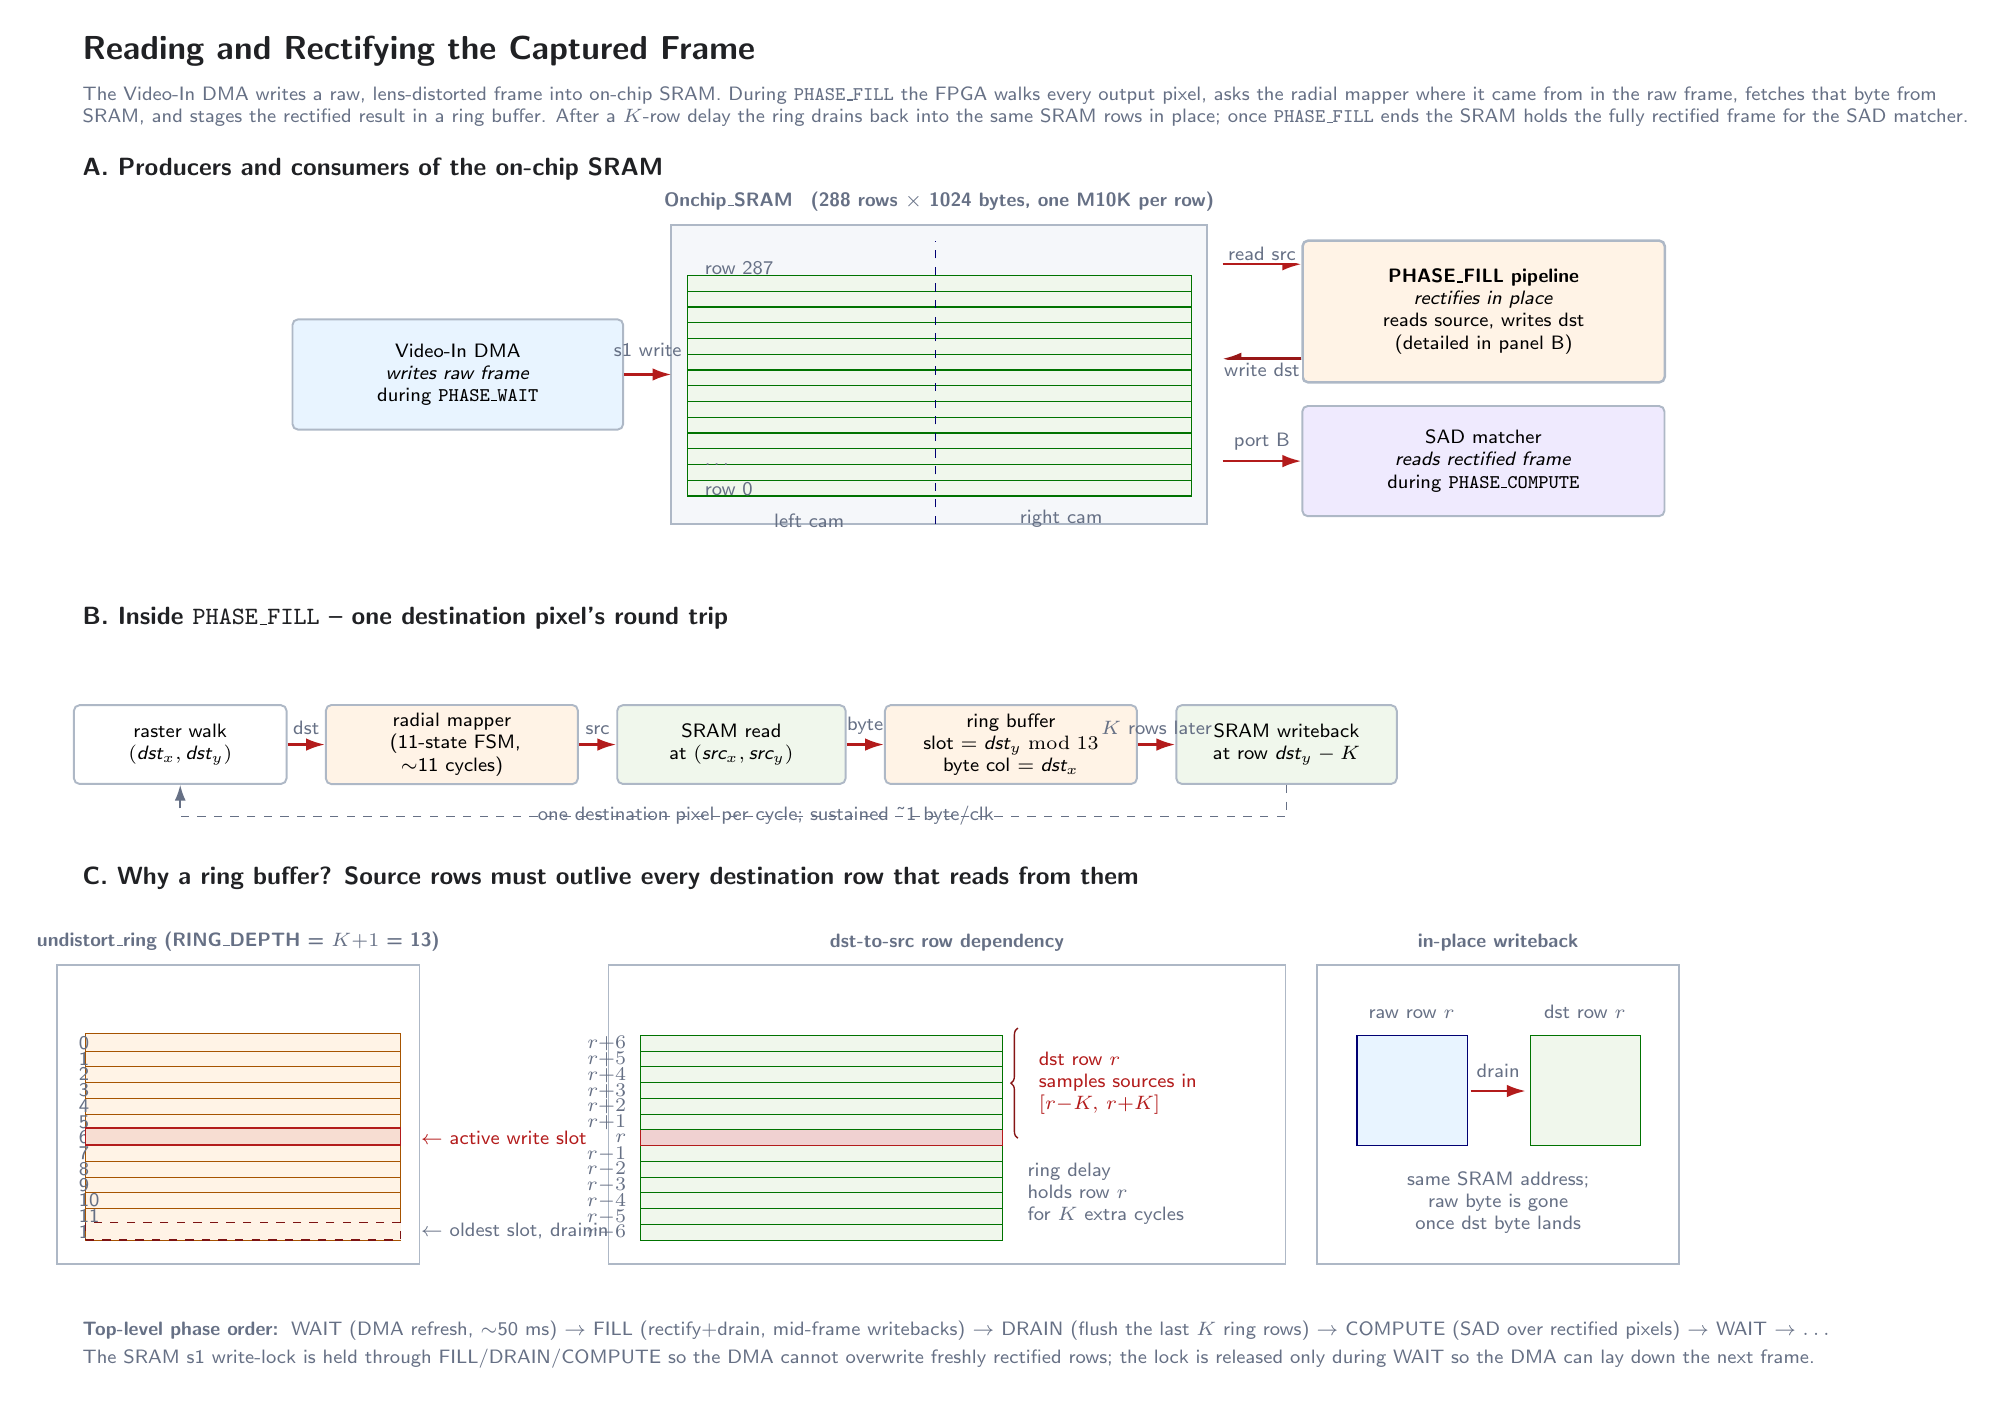
\begin{tikzpicture}[x=1mm,y=1mm,
  stage/.style={
    rectangle, rounded corners=2pt, draw=line, line width=0.7pt,
    fill=paper, align=center, font=\sffamily\scriptsize,
    inner xsep=3pt, inner ysep=3pt,
    minimum height=10mm
  },
  ramslot/.style={
    rectangle, draw=green!45!black, line width=0.4pt,
    fill=memory, minimum height=2.0mm, minimum width=64mm,
    inner sep=0pt
  },
  ringslot/.style={
    rectangle, draw=orange!65!black, line width=0.4pt,
    fill=compute, minimum height=2.2mm, minimum width=40mm,
    inner sep=0pt
  },
  pipe/.style={
    -{Latex[length=2.4mm,width=1.6mm]},
    draw=cornellred, line width=0.9pt
  },
  ghost/.style={
    -{Latex[length=2mm,width=1.4mm]},
    draw=muted, line width=0.6pt, dashed
  },
  axislbl/.style={font=\sffamily\scriptsize, text=muted}
]

  \node[title, anchor=west] at (0, 158) {Reading and Rectifying the Captured Frame};
  \node[labeltext, anchor=west, align=left] at (0, 151)
    {The Video-In DMA writes a raw, lens-distorted frame into on-chip SRAM.
     During \texttt{PHASE\_FILL} the FPGA walks every output pixel, asks the
     radial mapper where it came from in the raw frame, fetches that byte from\\
     SRAM, and stages the rectified result in a ring buffer. After a $K$-row
     delay the ring drains back into the same SRAM rows in place; once
     \texttt{PHASE\_FILL} ends the SRAM holds the fully rectified frame for the SAD matcher.};

  %====================================================================
  % SECTION A -- top-of-chip view: who reads/writes the SRAM
  %====================================================================
  \node[labeltext, anchor=west, text=ink, font=\sffamily\small\bfseries]
    at (0, 143) {A.\,\,Producers and consumers of the on-chip SRAM};

  % SRAM as a stack of rows (each row = one M10K)
  \begin{scope}[shift={(78, 100)}]
    \draw[fill=soft, draw=line, line width=0.7pt] (-2, -2) rectangle (66, 36);
    \node[labeltext, font=\sffamily\scriptsize\bfseries, anchor=south]
      at (32, 36.5) {Onchip\_SRAM \, (288 rows $\times$ 1024 bytes, one M10K per row)};
    \foreach \i in {0, 1, 2, 3, 4, 5, 6, 7, 8, 9, 10, 11, 12, 13} {
      \node[ramslot, anchor=south west] at (0, {2*\i + 1.5}) {};
    }
    \node[axislbl, anchor=west, font=\sffamily\scriptsize] at (1, 5.5) {\dots};
    \node[axislbl, anchor=west, font=\sffamily\scriptsize] at (1, 30.5) {row 287};
    \node[axislbl, anchor=west, font=\sffamily\scriptsize] at (1, 2.5) {row 0};
    \draw[blue!45!black, line width=0.3pt, dashed]
      (31.5, -2) -- (31.5, 34);
    \node[axislbl, anchor=south, font=\sffamily\scriptsize] at (15.5, -3.7) {left cam};
    \node[axislbl, anchor=south, font=\sffamily\scriptsize] at (47.5, -3.7) {right cam};
  \end{scope}

  % left: Video-In DMA writes raw frame
  \node[stage, anchor=east, minimum width=42mm, fill=camera, minimum height=14mm]
    (vdma) at (70, 117) {Video-In DMA\\\emph{writes raw frame}\\\scriptsize{}during \texttt{PHASE\_WAIT}};
  \draw[pipe] (vdma.east) -- (76, 117);
  \node[axislbl, font=\sffamily\scriptsize, anchor=south, align=center]
    at (73, 118) {s1 write};

  % right (upper): FILL pipeline reads + writes
  \node[stage, anchor=west, minimum width=46mm, fill=compute, minimum height=18mm,
        line width=0.9pt]
    (fill) at (156, 125) {\textbf{PHASE\_FILL pipeline}\\\emph{rectifies in place}\\\scriptsize{}reads source, writes dst\\\scriptsize{}(detailed in panel B)};
  % two arrows on opposite "halves" of the FILL-to-SRAM gap so their
  % heads don't pile up on top of each other.
  \draw[pipe] (146, 131) -- node[axislbl, above, font=\sffamily\scriptsize, fill=paper, inner sep=1pt]
        {read src} (156, 131);
  \draw[pipe, draw=cornellred!85!black] (156, 119) -- node[axislbl, below, font=\sffamily\scriptsize, fill=paper, inner sep=1pt]
        {write dst} (146, 119);

  % right (lower): SAD matcher reads via port B
  \node[stage, anchor=west, minimum width=46mm, fill=verify, minimum height=14mm]
    (sad) at (156, 106) {SAD matcher\\\emph{reads rectified frame}\\\scriptsize{}during \texttt{PHASE\_COMPUTE}};
  \draw[pipe] (146, 106) -- (156, 106);
  \node[axislbl, font=\sffamily\scriptsize, anchor=south, align=center,
        fill=paper, inner sep=1pt] at (151, 107) {port B};

  %====================================================================
  % SECTION B -- inside PHASE_FILL
  %====================================================================
  \node[labeltext, anchor=west, text=ink, font=\sffamily\small\bfseries]
    at (0, 86) {B.\,\,Inside \texttt{PHASE\_FILL} -- one destination pixel's round trip};

  % horizontal pipeline of boxes
  \node[stage, anchor=west, minimum width=27mm] (raster) at (0, 70)
    {raster walk\\$(\textit{dst}_x, \textit{dst}_y)$};
  \node[stage, anchor=west, minimum width=32mm, fill=compute] (mapper) at (32, 70)
    {radial mapper\\\scriptsize\,\,(11-state FSM,\\\scriptsize{}$\sim$11 cycles)};
  \node[stage, anchor=west, minimum width=29mm, fill=memory] (sramR) at (69, 70)
    {SRAM read\\at $(\textit{src}_x, \textit{src}_y)$};
  \node[stage, anchor=west, minimum width=32mm, fill=compute] (ring) at (103, 70)
    {ring buffer\\\scriptsize{}slot $=\textit{dst}_y \bmod 13$\\\scriptsize{}byte col $=\textit{dst}_x$};
  \node[stage, anchor=west, minimum width=28mm, fill=memory] (sramW) at (140, 70)
    {SRAM writeback\\\scriptsize{}at row $\textit{dst}_y - K$};

  \draw[pipe] (raster.east) -- node[axislbl, above, font=\sffamily\scriptsize]{dst} (mapper.west);
  \draw[pipe] (mapper.east) -- node[axislbl, above, font=\sffamily\scriptsize]{src} (sramR.west);
  \draw[pipe] (sramR.east) -- node[axislbl, above, font=\sffamily\scriptsize]{byte} (ring.west);
  \draw[pipe] (ring.east)  -- node[axislbl, above, font=\sffamily\scriptsize]{$K$ rows later} (sramW.west);

  % loop arrow showing 1 byte per cycle through the pipeline
  \draw[ghost] (sramW.south) -- ++(0,-4) -| (raster.south);
  \node[axislbl, font=\sffamily\scriptsize, anchor=north] at (88, 63.5)
    {one destination pixel per cycle; sustained \textasciitilde 1 byte/clk};

  %====================================================================
  % SECTION C -- the ring buffer, and why it's needed
  %====================================================================
  \node[labeltext, anchor=west, text=ink, font=\sffamily\small\bfseries]
    at (0, 53) {C.\,\,Why a ring buffer? Source rows must outlive every destination row that reads from them};

  % left: the ring buffer
  \begin{scope}[shift={(0, 6)}]
    \draw[draw=line, line width=0.6pt, fill=paper] (-2, -2) rectangle (44, 36);
    \node[labeltext, anchor=south, font=\sffamily\scriptsize\bfseries]
      at (21, 36.5) {undistort\_ring (RING\_DEPTH = $K{+}1$ = 13)};
    \foreach \i [count=\j from 0] in {12,11,10,9,8,7,6,5,4,3,2,1,0} {
      \pgfmathsetmacro{\ypos}{2*\j + 1}
      \node[ringslot, anchor=south west] at (1.5, \ypos) {};
      \node[axislbl, font=\sffamily\scriptsize, anchor=west] at (-0.5, {\ypos+1.1}) {\i};
    }
    % highlight the slot currently receiving writes
    \node[ringslot, anchor=south west, fill=compute!90!cornellred,
          draw=cornellred, line width=0.6pt] at (1.5, 13) {};
    \node[axislbl, anchor=west, font=\sffamily\scriptsize, text=cornellred]
      at (42.5, 14.1) {\,$\leftarrow$ active write slot};
    % highlight the slot being drained
    \node[ringslot, anchor=south west, fill=compute,
          draw=cornellred!70!black, line width=0.6pt, dashed] at (1.5, 1) {};
    \node[axislbl, anchor=west, font=\sffamily\scriptsize]
      at (42.5, 2.1) {\,$\leftarrow$ oldest slot, draining to SRAM};
  \end{scope}

  % middle: the dependency window
  \begin{scope}[shift={(70, 6)}]
    \draw[draw=line, line width=0.6pt, fill=paper] (-2, -2) rectangle (84, 36);
    \node[labeltext, anchor=south, font=\sffamily\scriptsize\bfseries]
      at (41, 36.5) {dst-to-src row dependency};

    % stack of source rows
    \foreach \i [count=\j from 0] in {r{-}6, r{-}5, r{-}4, r{-}3, r{-}2, r{-}1, r, r{+}1, r{+}2, r{+}3, r{+}4, r{+}5, r{+}6} {
      \pgfmathsetmacro{\ypos}{2*\j + 1}
      \pgfmathsetmacro{\isdst}{int(\j == 6)}
      \ifnum\isdst=1
        \node[rectangle, fill=cornellred!20, draw=cornellred, line width=0.5pt,
              minimum width=46mm, minimum height=2mm, anchor=south west,
              inner sep=0pt] at (2, \ypos) {};
      \else
        \node[rectangle, fill=memory, draw=green!45!black, line width=0.35pt,
              minimum width=46mm, minimum height=2mm, anchor=south west,
              inner sep=0pt] at (2, \ypos) {};
      \fi
      \node[axislbl, font=\sffamily\scriptsize, anchor=east] at (1.5, {\ypos+1}) {$\i$};
    }

    % brace showing the +/- K range
    \draw[decorate, decoration={brace, amplitude=2.5pt}, draw=cornellred!75!black,
          line width=0.5pt]
      (50, 14) -- node[axislbl, anchor=west, text=cornellred, font=\sffamily\scriptsize,
                       align=left, xshift=4pt] {dst row $r$\\samples sources in\\$[r{-}K,\,r{+}K]$} (50, 28);

    % annotation: keep row r alive until r+K processed
    \node[axislbl, anchor=west, font=\sffamily\scriptsize, align=left]
      at (50, 7) {ring delay\\holds row $r$\\for $K$ extra cycles};
  \end{scope}

  % right: the writeback timing diagram
  \begin{scope}[shift={(160, 6)}]
    \draw[draw=line, line width=0.6pt, fill=paper] (-2, -2) rectangle (44, 36);
    \node[labeltext, anchor=south, font=\sffamily\scriptsize\bfseries]
      at (21, 36.5) {in-place writeback};

    % before / after labels
    \node[axislbl, anchor=south, font=\sffamily\scriptsize] at (10, 28) {raw row $r$};
    \node[axislbl, anchor=south, font=\sffamily\scriptsize] at (32, 28) {dst row $r$};

    % colored boxes
    \node[rectangle, fill=camera, draw=blue!45!black, line width=0.5pt,
          minimum width=14mm, minimum height=14mm, anchor=south west,
          inner sep=0pt] at (3, 13) {};
    \node[rectangle, fill=memory, draw=green!45!black, line width=0.5pt,
          minimum width=14mm, minimum height=14mm, anchor=south west,
          inner sep=0pt] at (25, 13) {};

    \draw[pipe, line width=0.9pt] (17.5, 20) -- (24.5, 20);
    \node[axislbl, anchor=south, font=\sffamily\scriptsize] at (21, 20.5) {drain};

    \node[axislbl, anchor=north, align=center, font=\sffamily\scriptsize] at (21, 11)
      {same SRAM address;\\raw byte is gone\\once dst byte lands};
  \end{scope}

  %====================================================================
  % Footer / phase order
  %====================================================================
  \node[labeltext, anchor=north west, align=left] at (0, -2)
    {\textbf{Top-level phase order:}\, WAIT (DMA refresh, $\sim$50 ms)
     $\rightarrow$ FILL (rectify+drain, mid-frame writebacks)
     $\rightarrow$ DRAIN (flush the last $K$ ring rows)
     $\rightarrow$ COMPUTE (SAD over rectified pixels)
     $\rightarrow$ WAIT $\rightarrow\dots$\\[2pt]
     The SRAM s1 write-lock is held through FILL/DRAIN/COMPUTE so the DMA cannot
     overwrite freshly rectified rows; the lock is released only during WAIT so
     the DMA can lay down the next frame.};

\end{tikzpicture}
\end{document}
